% ============================================================
%  Dual-Pipeline Architecture — Conference Figure
%  Requires in preamble:
%    \usepackage{tikz}
%    \usetikzlibrary{arrows.meta,shapes.geometric,positioning,backgrounds,fit}
%    \pgfdeclarelayer{background}
%    \pgfsetlayers{background,main}
% ============================================================
 \usetikzlibrary{arrows.meta, backgrounds, positioning, fit}
\begin{figure}[tbp]

\centering
\resizebox{1.0\textwidth}{!}{%
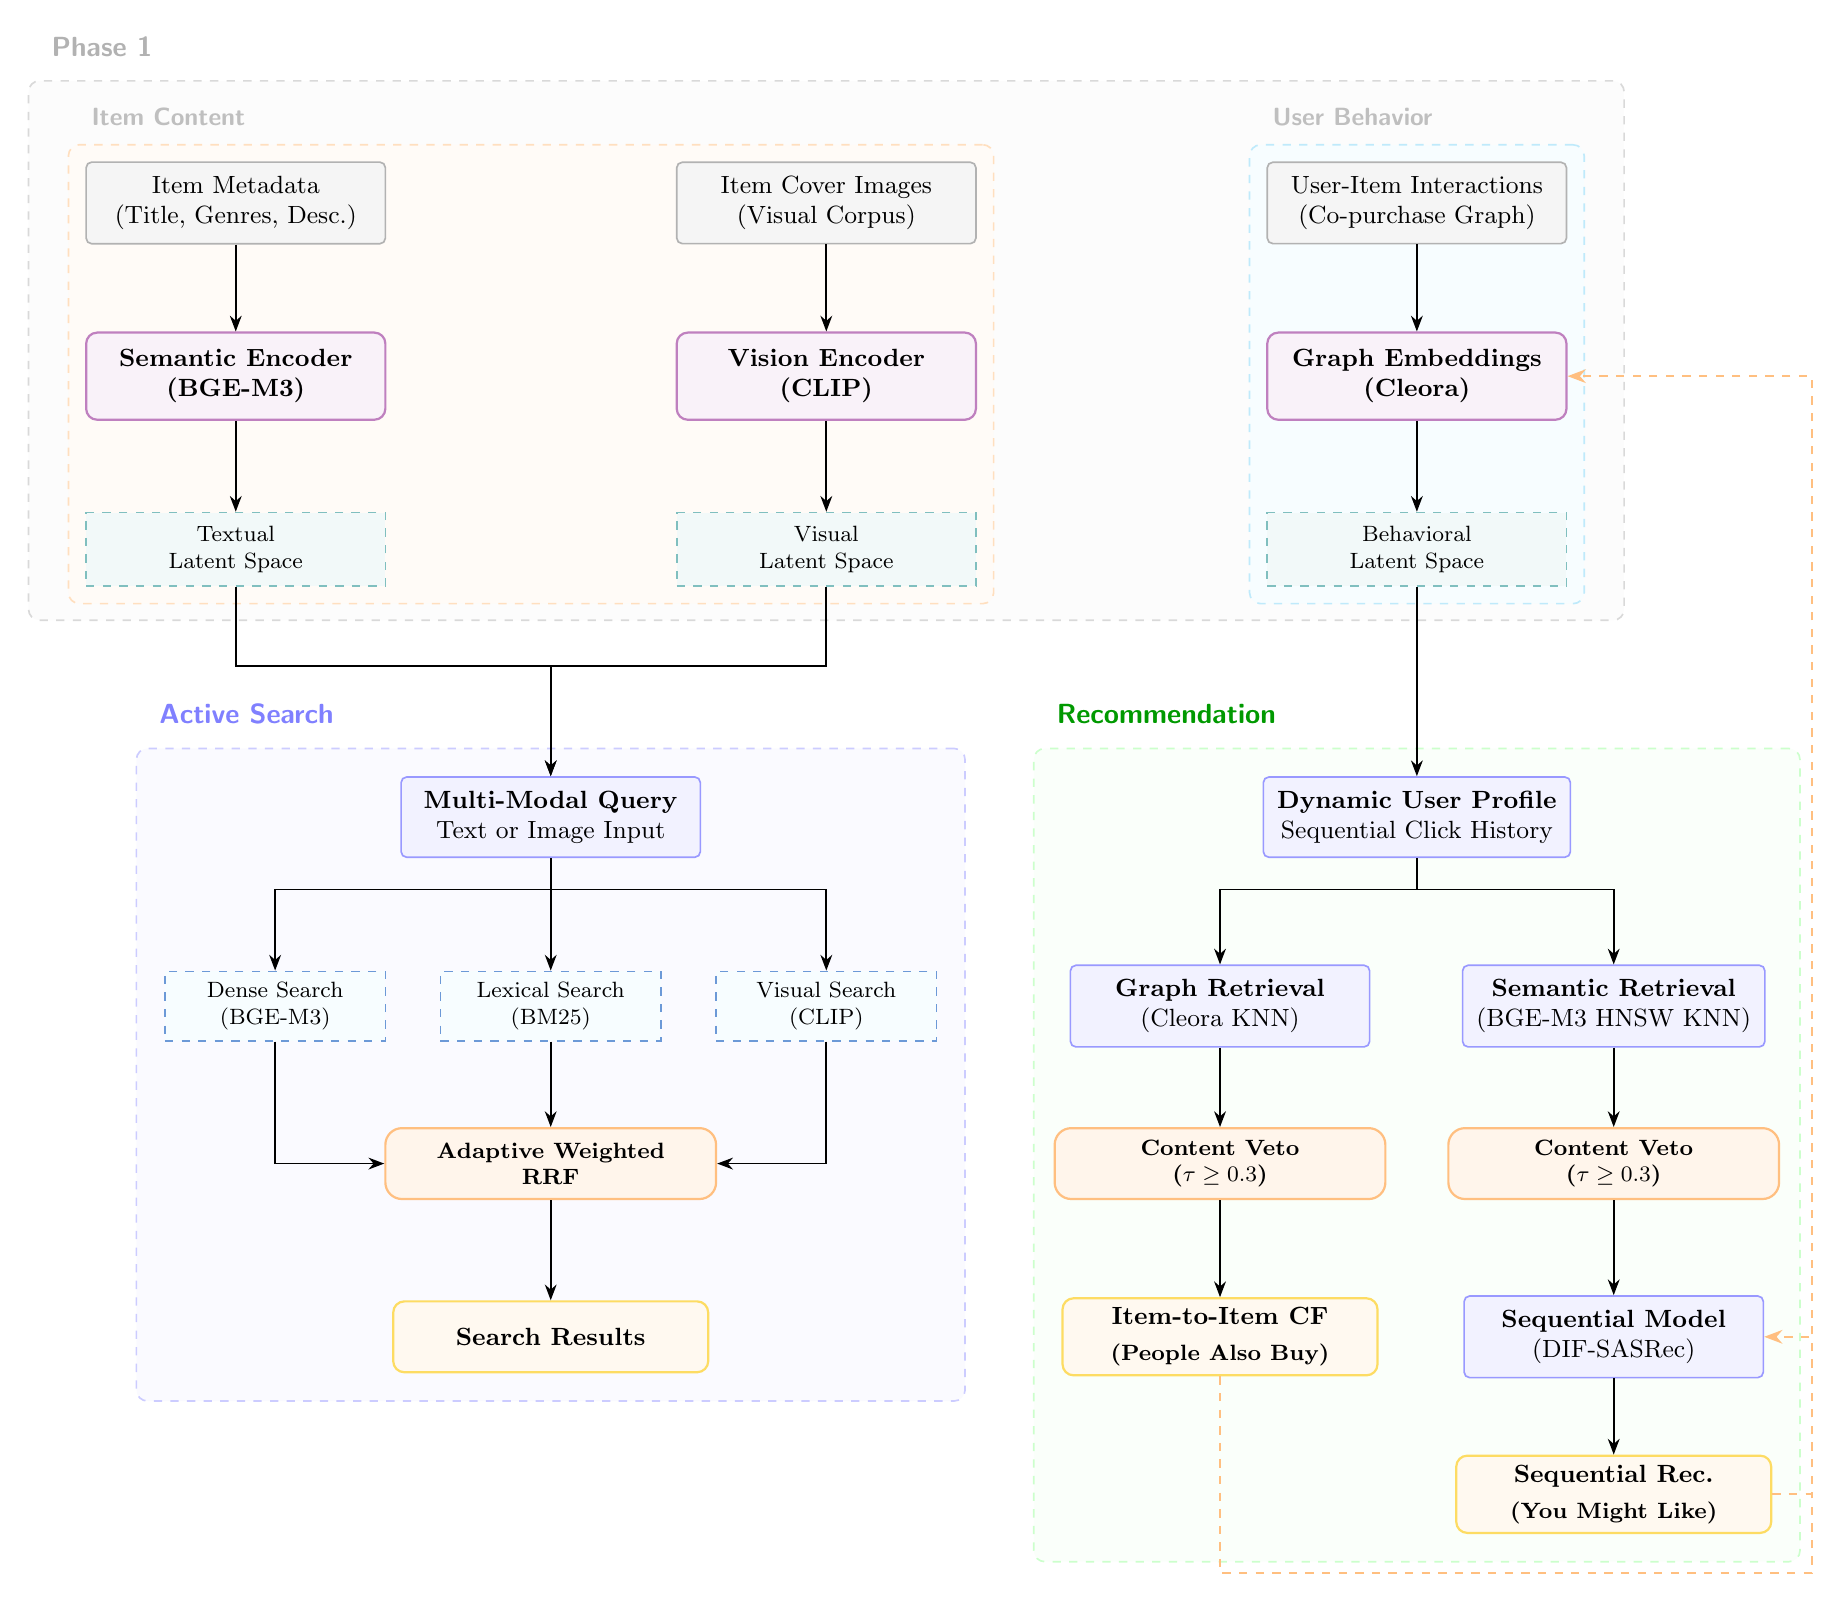
\begin{tikzpicture}[
  >=Stealth,
  every path/.style={line width=0.6pt},
  data/.style    ={draw=gray!60, fill=gray!8, rounded corners=2pt, align=center, inner sep=5pt, font=\small, minimum width=3.8cm, minimum height=1.0cm},
  model/.style   ={draw=violet!50, fill=violet!5, rounded corners=4pt, align=center, thick, inner sep=6pt, font=\small\bfseries, minimum width=3.8cm, minimum height=1.0cm},
  latent/.style  ={draw=teal!50, fill=teal!5, rectangle, align=center, dashed, inner sep=5pt, font=\footnotesize, minimum width=3.8cm, minimum height=0.9cm},
  task/.style    ={draw=blue!40, fill=blue!5, rounded corners=2pt, align=center, inner sep=5pt, font=\small, minimum width=3.8cm, minimum height=1.0cm},
  fusion/.style  ={draw=orange!50, fill=orange!8, rounded corners=6pt, thick, align=center, font=\footnotesize\bfseries, inner sep=4pt, minimum width=4.2cm, minimum height=0.9cm},
  retrieval/.style={draw=cyan!50!blue!60, fill=cyan!3, rectangle, align=center, dashed, inner sep=4pt, font=\footnotesize, minimum width=2.8cm, minimum height=0.8cm},
  output/.style  ={draw=yellow!60!orange!60, fill=yellow!10!orange!5, rounded corners=4pt, thick, align=center, font=\small\bfseries, minimum width=4.0cm, minimum height=0.9cm},
  label/.style   ={font=\scriptsize, text=gray!60, align=center}
]

% Coordinate definitions for easy adjustment
\def\pOneL{-7.5}
\def\pOneC{0.0}
\def\pOneR{7.5}

\def\colPhaseA{-7.5}
\def\colPhaseB{7.5}
\def\colRecL{5.0}
\def\colRecR{10.0}

\def\rowData{0}
\def\rowModel{-2.2}
\def\rowLatent{-4.4}
\def\rowTask{-7.8}
\def\rowPipe{-10.2}
\def\rowVeto{-12.2}
\def\rowOut{-14.4}
\def\rowOutB{-16.4}      % Pipeline B extra depth (DIF-SASRec + YML)

% ==========================================
% PHASE 1: Representation Learning
% ==========================================

\node[data]   (d_text)   at (\pOneL, \rowData)  {Item Metadata\\(Title, Genres, Desc.)};
\node[model]  (m_bge)    at (\pOneL, \rowModel) {Semantic Encoder\\(BGE-M3)};
\node[latent] (l_sem)    at (\pOneL, \rowLatent){Textual\\Latent Space};

\node[data]   (d_img)    at (\pOneC, \rowData)  {Item Cover Images\\(Visual Corpus)};
\node[model]  (m_clip)   at (\pOneC, \rowModel) {Vision Encoder\\(CLIP)};

\node[latent] (l_vis)    at (\pOneC, \rowLatent){Visual\\Latent Space};

\node[data]   (d_graph)  at (\pOneR, \rowData)  {User-Item Interactions\\(Co-purchase Graph)};
\node[model]  (m_cleora) at (\pOneR, \rowModel) {Graph Embeddings\\(Cleora)};

\node[latent] (l_behav)  at (\pOneR, \rowLatent){Behavioral\\Latent Space};

\draw[->] (d_text) -- (m_bge);   \draw[->] (m_bge)    -- (l_sem);
\draw[->] (d_img)  -- (m_clip);  \draw[->] (m_clip)   -- (l_vis);
\draw[->] (d_graph)-- (m_cleora);\draw[->] (m_cleora) -- (l_behav);

% Spacers to extend Phase 1 box for sub-box containment
\coordinate (bg_rep_top)   at ([yshift=0.6cm]d_text.north);
\coordinate (bg_rep_left)  at ([xshift=-0.3cm]d_text.west);
\coordinate (bg_rep_right) at ([xshift=0.3cm]d_graph.east);


% ==========================================
% PHASE 2A: Active Search
% ==========================================

% Column coordinates for three-channel retrieval layout
\def\colSearchQ{-3.5}           % Query node (centre of channels)
\def\colSearchL{-7.0}           % BGE-M3 HNSW
\def\colSearchC{-3.5}           % Tantivy BM25
\def\colSearchR{0.0}            % CLIP HNSW
\def\colSearchOut{-3.5}         % RRF + output (centre of channels)

\node[task]   (t_search)   at (\colSearchQ, \rowTask) {\textbf{Multi-Modal Query}\\Text or Image Input};

% Three parallel retrieval channels
\node[retrieval] (r_text)  at (\colSearchL, \rowPipe) {Dense Search\\(BGE-M3)};
\node[retrieval] (r_kw)    at (\colSearchC, \rowPipe) {Lexical Search\\(BM25)};
\node[retrieval] (r_vis)   at (\colSearchR, \rowPipe) {Visual Search\\(CLIP)};


\node[fusion] (f_rrf)   at (\colSearchOut, \rowVeto) {Adaptive Weighted\\RRF};
\node[output] (out_search) at (\colSearchOut, \rowOut) {Search Results};

% Incoming queries from latent spaces (Phase 1) — converge at t_search.north
\draw[->] (l_sem.south) -- ++(0,-1.0) -| (t_search.north);
\draw[->] (l_vis.south) -- ++(0,-1.0) -| (t_search.north);

% Query → Retrieval channels
\draw[->] (t_search.south) -- ++(0,-0.4) -| (r_text.north);
\draw[->] (t_search.south) -- ++(0,-0.4) -| (r_kw.north);
\draw[->] (t_search.south) -- ++(0,-0.4) -| (r_vis.north);

% Channels → RRF
\draw[->] (r_text.south) |- (f_rrf.west);
\draw[->] (r_kw.south)   -- (f_rrf.north);
\draw[->] (r_vis.south)  |- (f_rrf.east);

% RRF → Output
\draw[->] (f_rrf) -- (out_search);


% ==========================================
% PHASE 2B: Recommendation
% ==========================================

\node[task]   (t_profile) at (\colPhaseB, \rowTask) {\textbf{Dynamic User Profile}\\Sequential Click History};

\node[task]   (p_collab) at (\colRecL, \rowPipe) {\textbf{Graph Retrieval}\\(Cleora KNN)};
\node[fusion] (f_veto)   at (\colRecL, \rowVeto) {Content Veto\\($\tau \geq 0.3$)};
\node[output] (out_pab)  at (\colRecL, \rowOut)  {Item-to-Item CF\\[2pt]\footnotesize{(People Also Buy)}};

\node[task]   (p_retrv)  at (\colRecR, \rowPipe) {\textbf{Semantic Retrieval}\\(BGE-M3 HNSW KNN)};
\node[fusion] (f_veto_b) at (\colRecR, \rowVeto) {Content Veto\\($\tau \geq 0.3$)};
\node[task]   (p_seq)    at (\colRecR, \rowOut) {\textbf{Sequential Model}\\(DIF-SASRec)};
\node[output] (out_yml)  at (\colRecR, \rowOutB)  {Sequential Rec.\\[2pt]\footnotesize{(You Might Like)}};

\draw[->] (l_behav.south) -- (t_profile.north);
\draw[->] (t_profile.south) -- ++(0,-0.4) -| (p_collab.north);
\draw[->] (t_profile.south) -- ++(0,-0.4) -| (p_retrv.north);
\draw[->] (p_collab) -- (f_veto);
\draw[->] (f_veto)   -- (out_pab);
\draw[->] (p_retrv)  -- (f_veto_b);
\draw[->] (f_veto_b) -- (p_seq);
\draw[->] (p_seq)    -- (out_yml);


% ==========================================
% DEPENDENCIES & FEEDBACK LOOPS
% ==========================================


% Online feedback loops
\draw[->, thick, dashed, orange!50] (out_yml.east)  -- ++(0.5,0) |- (p_seq.east);

% PAB → trunk (south below SML, then right to trunk) — joins trunk without arrow
\draw[thick, dashed, orange!50] (out_pab.south) -- ++(0,-2.5) -| ([xshift=0.5cm]out_yml.east);
% SML → trunk (right, then up to Cleora) — carries arrow
\draw[->, thick, dashed, orange!50] (out_yml.east)  -- ++(0.5,0) |- (m_cleora.east);


% ==========================================
% BACKGROUND BOUNDING BOXES
% ==========================================

\begin{pgfonlayer}{background}
  \node[draw=gray!30, fill=gray!2, rounded corners, dashed, inner sep=12pt,
        fit=(d_text)(d_graph)(l_sem)(l_vis)(l_behav)(m_clip)(bg_rep_top)(bg_rep_left)(bg_rep_right)] (bg_rep) {};
  \node[draw=orange!25, fill=orange!3, dashed, inner sep=6pt, rounded corners=4pt,
        fit=(d_text)(m_bge)(l_sem)(d_img)(m_clip)(l_vis)] (bg_content) {};
  \node[draw=cyan!25, fill=cyan!3, dashed, inner sep=6pt, rounded corners=4pt,
        fit=(d_graph)(m_cleora)(l_behav)] (bg_behavior) {};
  \node[draw=blue!20, fill=blue!2, rounded corners, dashed, inner sep=10pt,
        fit=(t_search)(r_text)(r_vis)(out_search)] (bg_search) {};
  \node[draw=green!20, fill=green!2, rounded corners, dashed, inner sep=10pt,
        fit=(t_profile)(out_pab)(out_yml)] (bg_rec) {};
        
  \node[anchor=south west, font=\sffamily\bfseries\color{gray!60}]
        at ([xshift=5pt, yshift=5pt]bg_rep.north west)       {Phase 1};
  \node[anchor=south west, font=\sffamily\bfseries\small\color{gray!50}]
        at ([xshift=5pt, yshift=3pt]bg_content.north west)   {Item Content};
  \node[anchor=south west, font=\sffamily\bfseries\small\color{gray!50}]
        at ([xshift=5pt, yshift=3pt]bg_behavior.north west)  {User Behavior};
  \node[anchor=south west, font=\sffamily\bfseries\color{blue!50}]
        at ([xshift=5pt, yshift=5pt]bg_search.north west) {Active Search};
  \node[anchor=south west, font=\sffamily\bfseries\color{green!60!black}]
        at ([xshift=5pt, yshift=5pt]bg_rec.north west)    {Recommendation};
\end{pgfonlayer}

\end{tikzpicture}%
}
\caption{System architecture (data-flow view).}%

\label{fig:arch}
\end{figure}
